\documentclass[9pt,t]{beamer}
\usetheme{Wisconsin}
\usepackage[utf8]{inputenc}
\setbeamertemplate{page number in head/foot}[totalframenumber]
\setbeamerfont{title}{size=\LARGE}
\setbeamerfont{subtitle}{size=\Large}
\setbeamerfont{block body}{size=\footnotesize}
\setbeamerfont{author}{size=\LARGE}
\setbeamerfont{date}{size=\Large}
\setlength{\leftmargini}{0pt}

%subcaptions
\usepackage{subcaption}
% \captionsetup[subfigure]{labelformat=empty} % turn off labeling figures

% turn off Figure in captions
\usepackage{caption}
% \captionsetup[figure]{labelformat=empty}

\newcommand{\QOR}{\qquad \text{OR} \qquad}
\newcommand{\QAND}{\qquad \text{AND} \qquad}
\newcommand{\QTHUS}{\qquad \text{THUS} \qquad}
\newcommand{\QTHEN}{\qquad \text{THEN} \qquad}
\newcommand{\QWITH}{\qquad \text{WITH} \qquad}
\newcommand{\QFOR}{\qquad \text{FOR} \qquad}
\newcommand{\QSO}{\qquad \text{SO} \qquad}
\newcommand{\QWHERE}{\qquad \text{WHERE} \qquad}
\newcommand{\LINE}{\par\noindent\rule{\textwidth}{0.4pt}\par}
\newcommand{\toinf}{\rightarrow\infty}
\newcommand{\tozero}{\rightarrow0}
\newcommand{\qeq}{\overset{?}{=}}
\newcommand{\ceq}{\overset{\checkmark}{=}}
\renewcommand{\epsilon}{\varepsilon}


% Roman Numerals
\newcommand{\rom}[1]{\expandafter\uppercase{\Romannumeral #1\relax}}

% hypersetup
\usepackage{hyperref}
\hypersetup{colorlinks,
            linkcolor = white,
            citecolor = white,
            urlcolor = cyan
}


\def\brac#1{\{#1\}}
\def\Brac#1{\big\{#1\big\}}
\def\BRAC#1{\bigg\{#1\bigg\}}
\def\angbrac#1{\langle#1\rangle}
\def\Angbrac#1{\big\langle#1\big\rangle}
\def\ANGBRAC#1{\bigg\langle#1\bigg\rangle}

% % Transitional slides between sections
% \AtBeginSection[]
% {
%     \begin{frame}
%         \frametitle{Table of Contents}
%         \tableofcontents[currentsection]
%     \end{frame}
% }


% Bibliography
\usepackage[sorting=none]{biblatex} %Imports biblatex package and cites in order of appearance
\addbibresource{mc2023_pres.bib} %Import the bibliography file
% make all font colors white
\setbeamercolor{bibliography item}{fg=white}
\setbeamercolor{bibliography entry author}{fg=white}
\setbeamercolor{bibliography entry title}{fg=white}
\setbeamercolor{bibliography entry location}{fg=white}
\setbeamercolor{bibliography entry note}{fg=white}
% adds numeric labels linked to bib entries
\setbeamertemplate{bibliography item}{\insertbiblabel}

% eliminate header within an environment
\makeatletter
    \newenvironment{withoutheadline}{
       \setbeamertemplate{headline}[default]
       \def\beamer@entrycode{\vspace*{-\headheight}}
    }{}
\makeatother

\title{Verification of the Cardinal Multiphysics Solver}
\subtitle{1-D Coupled Heat Transfer and Neutron Transport}
\author{Lewis Gross, April J. Novak, Patrick Shriwise, and Paul P.H. Wilson\vspace*{-1cm}}
\date{August 15, 2022}
%%----------------------------------------------------------------------------%%
\begin{document}

\begin{withoutheadline}
\begin{frame}[plain] % the plain makes the first frame look good
    \maketitle
\end{frame}
\end{withoutheadline}

%%----------------------------------------------------------------------------%%
%% Overview
%%----------------------------------------------------------------------------%%
\begin{withoutheadline}
\begin{frame}{Outline}
  \tableofcontents
\end{frame}
\end{withoutheadline}


%%----------------------------------------------------------------------------%%
%% Section 1
%%----------------------------------------------------------------------------%%
\section{Introduction}
\begin{frame}{Introduction}
    \begin{itemize}
        \item Nuclear systems have many types of physics that are coupled!
        \item Multiphysics simulations are becoming more and more popular.
        \item Cardinal - our software choice
        \item High burden of proof to design systems. The tools we use need V\&V to gain trustworthiness.
        \item Verification via analytical benchmarks allow measurement of true accuracy for numerical simulation.
        \item Greisheimer and Kooreman 1-D presented an analytical benchmark that features coupled heat transfer
              and neutron transport \cite{analytical-benchmark}.
    \end{itemize}
\end{frame}


%%----------------------------------------------------------------------------%%
%% Section 2
%%----------------------------------------------------------------------------%%
\section{Analytical Benchmark}
\begin{frame}{Analytical Benchmark}
    \begin{itemize}
        \item This analytical benchmark includes $S_2$ transport, Doppler-broadened cross sections, 1-D thermal conduction
        and expansion, and convective boundary conditions.
        \begin{itemize}
            \item $S_{2}$ transport restricts particles to move in the $\pm$x direction; or $\mu=\cos\theta=\pm 1$.
            \item Doppler-broadening
            \begin{equation}\label{doppler-micro-xs}
                \sigma_{t}(x) = \sigma_{t,0}\sqrt{\frac{T_{0}}{T(x)}}.
            \end{equation}
            \item 1-D thermal expansion
            \begin{equation} \label{density-temp-relation}
                \rho(x) =  \rho_{0} \sqrt{\frac{T_{0}}{T(x)}}.
            \end{equation}
            \item Linear temperature dependence on thermal conductivity
            \begin{equation}\label{thermal-conductivity-temp-relation}
                \kappa(x) = \kappa_{0} T(x)
            \end{equation}
        \end{itemize}
        \item The conduction equation governs energy conservation in the slab and can be described in terms of the thermal conductivity
        $\kappa$, the energy released \textbf{per reaction} $q$, the total macroscopic cross section $\Sigma_{t}$, and the neutron flux $\phi$,
        \begin{equation}
            \frac{d}{dx}\left\lbrack\kappa(T)\frac{dT(x)}{dx}\right\rbrack + q \Sigma_{t}(x)\phi(x) = 0.
        \end{equation}
    \end{itemize}
\end{frame}

\begin{frame}{Analytical Benchmark}
    \begin{itemize}
        \item Based on 1-D $S_{2}$ transport, the neutron flux is governed body
        \begin{equation}
            \frac{\partial}{\partial x}\bigg[\frac{1}{\Sigma_{t}(x)} \frac{\partial\phi(x)}{\partial x} \bigg] + \Sigma_{t}(x)
            \big(\lambda - 1\big)\phi(x) = 0
        \end{equation}
        \item where $\lambda \equiv (\frac{1}{k_{eff}}\frac{\nu \Sigma_{f}}{\Sigma_{t}} + \frac{\Sigma_{s}}{\Sigma_{t}} )$ is
        the combined in-scattering and quasi-static fission source term \cite{analytical-benchmark}.
        \item Using (\ref{doppler-micro-xs}) and (\ref{density-temp-relation}) gives a Doppler-broadened, macroscopic, total
              cross section that accounts for changes in density due to temperature as
        \begin{equation}\begin{aligned}
            \Sigma_{t}(x) =&\  \frac{\rho_{0}\sigma_{t,0} N_{A}}{A} \frac{T_{0}}{T(x)}\\
            =&\  \Sigma_{t,0}\frac{T_{0}}{T(x)} ,
        \end{aligned}\end{equation}
        where $ \sigma_{t,0}$ is the total microscopic cross section at $T_{0}$, $N_{A}$ is Avogadro's number, and $A$ is the mass number
        of the medium.
    \end{itemize}
\end{frame}


\begin{frame}{System Domain, Differential Equations, and Boundary Conditions}
    \begin{figure}[H]
        \centering
        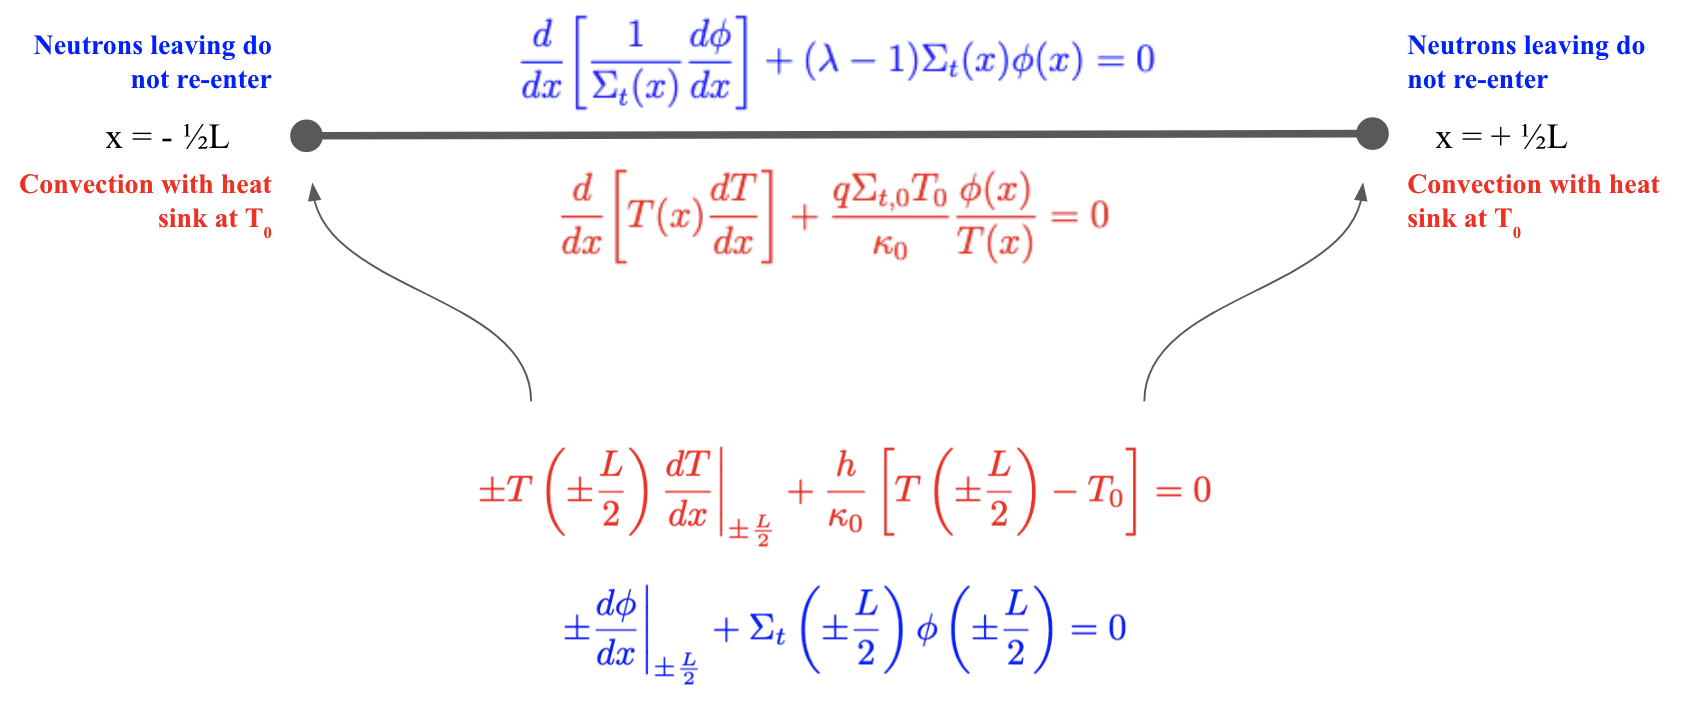
\includegraphics[width=0.775\linewidth]{figures/1D_Benchmark_Diagram.png}
    \end{figure}
    \begin{itemize}
        \item The fundamental assumption of \cite{analytical-benchmark} is that: $T(x)=f\phi(x)$. This imposes
        two constraints that determine the system heat transfer coefficient $h$ and the total microscopic
        cross section $\sigma_{t,0}$. The solution that satisfies the above is given by
        \begin{equation}
            \phi(x) = \phi(0) \sqrt{1 - \frac{(\lambda - 1)P^{2}x^{2}}{L^{2}q^{2}\phi^2(0)}}
        \end{equation}
        where $P$ is the slab power and $L$ is the slab equilibrium length.
    \end{itemize}
\end{frame}

%%----------------------------------------------------------------------------%%
%% Section 3
%%----------------------------------------------------------------------------%%
\section{Computational Model}
\begin{frame}{OpenMC Model}
    \begin{itemize}
        \item Fictitious material but we can define its XS, HTC, etc.
    \end{itemize}
\end{frame}

\begin{frame}{MOOSE Heat Conduction Model}
    \begin{itemize}
        \item
    \end{itemize}
\end{frame}

\begin{frame}{Coupling, Data Mapping, and Convergence Criteria}
    \begin{itemize}
        \item
    \end{itemize}
\end{frame}


%%----------------------------------------------------------------------------%%
%% Section 4
%%----------------------------------------------------------------------------%%
\section{Results and Discussion}
\begin{frame}{Outputs and Comparisons}
    \begin{itemize}
        \item results
    \end{itemize}
\end{frame}

\begin{frame}{Future and companion work}
    \begin{itemize}
        \item discuss
    \end{itemize}
\end{frame}

%%----------------------------------------------------------------------------%%
%% Bibliography
%%----------------------------------------------------------------------------%%

\begin{frame}{Cite Dump}
    \begin{itemize}
        \item \cite{aya2023} \cite{brown-entropy-2006} \cite{dufek} \cite{lindsay2022moose} \cite{nekrs} \cite{novak-2023} \cite{novak2022-cardinal} \cite{openmc}
    \end{itemize}
\end{frame}

\begin{withoutheadline}
\begin{frame}[allowframebreaks]{Bibliography}
    \printbibliography
\end{frame}
\end{withoutheadline}

\begin{withoutheadline}
    \begin{frame}{Acknowledgements}
        \begin{itemize}
            \item Co-authors: April J. Novak, Patrick Shriwise, Paul P.H. Wilson
            \item OpenMC, Cardinal, and MOOSE teams!
        \end{itemize}
        \begin{figure}[H]
            \centering
            
\includegraphics[width=0.8\linewidth]{figures/openmc_logo.png}
        \end{figure}
        \begin{figure}[H]
            \centering
            
\includegraphics[width=0.8\linewidth]{figures/cardinal_logo.png}
        \end{figure}
        \begin{figure}[H]
            \centering
            
\includegraphics[width=0.8\linewidth]{figures/moose_logo.png}
        \end{figure}
    \end{frame}
\end{withoutheadline}

\begin{withoutheadline}
\begin{frame}[allowframebreaks]{Extra Content and Derivations}
    \begin{itemize}
        \item Going from the steady-state, mono-energetic, 1-D neutron transport equation to the ODE that describes neutron transport for this benchmark:
        \begin{equation}
            \mu \frac{\partial \psi(x,\mu)}{\partial x} + \Sigma_{t}(x)\psi(x,\mu) =
            \int_{-1}^{1} \frac{1}{2}\big[\Sigma_{s}(x) + \frac{\nu \Sigma_{f}(x)}{k_{eff}}\big] \psi(x,\mu')d\mu'
        \end{equation}
        For now, lump the fission term into the scattering cross section to get
        \begin{equation} \label{transport eq}
            \mu \frac{\partial \psi(x,\mu)}{\partial x} + \Sigma_{t}(x)\psi(x,\mu) =
            \int_{-1}^{1} \frac{1}{2}\Sigma_{s}(x) \psi(x,\mu')d\mu'
        \end{equation}
        Define the scalar flux and the magnitude of current
        \begin{equation}
            \phi(x) = \int_{-1}^{1} \psi(x,\mu) d\mu \QAND J(x) = \int_{-1}^{1} \mu \psi(x,\mu) d\mu.
        \end{equation}
        Considering $S_{2}$ transport means restricting the angular cosine to $\mu = \pm 1$:
        \begin{equation}
            \psi(x,\mu) = \psi(x,-1) \delta(\mu+1) + \psi(x,1) \delta(\mu-1)
        \end{equation}
        (sometimes denoted $\psi^{+}\equiv \psi(x,1) \delta(\mu-1) $ and $\psi^{-}\equiv \psi(x,-1) \delta(\mu+1) $)
        \newpage
        Now carrying out the integral definitions with $S_{2}$ quantities gives
        \begin{equation} \label{scalar flux}
            \phi(x) = \int_{-1}^{1} \bigg[ \psi(x,-1) \delta(\mu+1) + \psi(x,1) \delta(\mu-1) \bigg]d\mu =
            \psi(x,-1) + \psi(x,1)
        \end{equation}
        and
        \begin{equation} \label{current}
            J(x) = \int_{-1}^{1} \mu \bigg[ \psi(x,-1) \delta(\mu+1) + \psi(x,1) \delta(\mu-1) \bigg] d\mu =
            \psi(x,1) - \psi(x,-1)
        \end{equation}
        Evaluating (\ref{transport eq}) at $\mu=\pm 1$ gives
        \begin{equation} \label{-1}
            -\frac{\partial \psi(x,-1)}{\partial x} + \Sigma_{t}(x)\psi(x,-1) =
            \frac{1}{2}\Sigma_{s}(x) \phi(x);
        \end{equation}
        \begin{equation} \label{+1}
            \frac{\partial \psi(x,1)}{\partial x} + \Sigma_{t}(x)\psi(x,1) =
            \frac{1}{2}\Sigma_{s}(x) \phi(x).
        \end{equation}
        Adding (\ref{-1}) and (\ref{+1}) gives
        \begin{equation}\label{sum}
            -\frac{\partial \psi(x,-1)}{\partial x} +  \frac{\partial \psi(x,1)}{\partial x} + \Sigma_{t}(x)\big(\psi(x,-1) + \psi(x,1) \big) =
            \Sigma_{s}(x) \phi(x)
        \end{equation}
        The results for $\phi(x)$ and $J(x)$ can simplify (\ref{sum})
        \begin{equation}  \label{current derivative}
            \frac{\partial J(x)}{\partial x} + \Sigma_{t}(x)\phi(x) =
            \Sigma_{s}(x) \phi(x)
        \end{equation}
        Subtracting  (\ref{-1}) and (\ref{+1}) gives
        \begin{equation}
            -\frac{\partial \psi(x,-1)}{\partial x}
            - \frac{\partial \psi(x,1)}{\partial x} + \Sigma_{t}(x)\big(\psi(x,-1)  - \Sigma_{t}(x)\psi(x,1)\big) =
            0
        \end{equation}
        Which can be transformed with similar tricks to
        \begin{equation} \label{flux derrivative}
            \frac{\partial\phi(x)}{\partial x} + \Sigma_{t}(x)J(x) = 0 \QOR
            J(x) = - \frac{1}{\Sigma_{t}(x)} \frac{\partial\phi(x)}{\partial x}
        \end{equation}
        Since $\frac{\partial J(x)}{\partial x}$ appears in (\ref{current derivative}), we can take the derivative of both sides of (\ref{flux derrivative}) and substitute it in
        \begin{equation}
          \frac{\partial J(x)}{\partial x} =
          - \frac{\partial}{\partial x} \bigg[ \frac{1}{\Sigma_{t}(x)} \frac{\partial\phi(x)}{\partial x} \bigg]
        \end{equation}
        Now the equation that only depends on $\phi(x)$ is given by
        \begin{equation}
            -\frac{\partial}{\partial x}\bigg[\frac{1}{\Sigma_{t}(x)} \frac{\partial\phi(x)}{\partial x} \bigg] + \Sigma_{t}(x)\phi(x) =
            \Sigma_{s}(x) \phi(x)
        \end{equation}
        At this point, we ``un-lump" the scattering cross section to write out the fission term
        \begin{equation}
            -\frac{\partial}{\partial x}\bigg[\frac{1}{\Sigma_{t}(x)} \frac{\partial\phi(x)}{\partial x} \bigg] + \Sigma_{t}(x)\phi(x) =
            \bigg[\Sigma_{s}(x) + \frac{\nu \Sigma_{f}}{k_{eff}}\bigg]\phi(x)
        \end{equation}
        \begin{equation}
            -\frac{\partial}{\partial x}\bigg[\frac{1}{\Sigma_{t}(x)} \frac{\partial\phi(x)}{\partial x} \bigg] + \Sigma_{t}(x)
            \bigg[1 - \frac{\Sigma_{s}(x) + \frac{\nu \Sigma_{f}}{k_{eff}}}{\Sigma_{t}}\bigg]\phi(x) = 0
        \end{equation}
        \begin{equation}
            \frac{\partial}{\partial x}\bigg[\frac{1}{\Sigma_{t}(x)} \frac{\partial\phi(x)}{\partial x} \bigg] + \Sigma_{t}(x)
            \bigg[\frac{\Sigma_{s}(x) + \frac{\nu \Sigma_{f}}{k_{eff}}}{\Sigma_{t}} - 1\bigg]\phi(x) = 0
        \end{equation}
        Now define
        \begin{equation}
            \lambda \equiv \frac{\Sigma_{s}(x) + \frac{\nu \Sigma_{f}}{k_{eff}}}{\Sigma_{t}}
        \end{equation}
        giving the final result:
        \begin{equation}
            \frac{\partial}{\partial x}\bigg[\frac{1}{\Sigma_{t}(x)} \frac{\partial\phi(x)}{\partial x} \bigg] + \Sigma_{t}(x)
            \big(\lambda - 1\big)\phi(x) = 0
        \end{equation}
        \newpage
        The next task is to apply boundary conditions so that $\phi(x)$ can be specified. In discrete ordinates with $\mu=\pm1$ ($S_{2}$), we use the vacuum boundary condition. The angular flux for positive angular cosines is zero at the left boundary and is zero for negative angular cosines at the right boundary.
        Using the previous results for $\phi(x)$ and $J(x)$ at the boundaries gives
        \begin{multline}
            \phi(x=\frac{L}{2}) =  \psi(x=\frac{L}{2},\mu =-1) + \psi(x=\frac{L}{2},\mu =1) \QAND  \\ \phi(x=-\frac{L}{2}) =  \psi(x=-\frac{L}{2},\mu =-1) + \psi(x=-\frac{L}{2},\mu =1)
        \end{multline}
        and
        \begin{multline}
            J(x=\frac{L}{2}) = - \psi(x=\frac{L}{2},-1)  + \psi(x=\frac{L}{2},1) \QAND \\ J(x=-\frac{L}{2}) = - \psi(x=-\frac{L}{2},-1)  + \psi(x=-\frac{L}{2},1)
        \end{multline}
        Now, terms can be crossed out due to vacuum boundaries. This gives that
        \begin{multline}
            \phi(x=\frac{L}{2}) =  \psi(x=\frac{L}{2},\mu =1) \QAND \\ \phi(x=-\frac{L}{2}) =  \psi(x=-\frac{L}{2},\mu =-1)
        \end{multline}
        \begin{multline}
            J(x=\frac{L}{2}) = \psi(x=\frac{L}{2},\mu =1) \QAND \\ J(x=-\frac{L}{2}) = - \psi(x=-\frac{L}{2},\mu =-1)
        \end{multline}
        Using this with (\ref{flux derrivative}) gives the desired boundary conditions
        \begin{equation}
            J(x=\pm \frac{L}{2}) = \pm \phi(x=\pm \frac{L}{2})
        \end{equation}
        And the boundary conditions of interest are now
        \begin{equation}
            \frac{\partial\phi}{\partial x}\bigg|_{x=\pm \frac{L}{2}} \pm  \Sigma_{t}(x=\pm \frac{L}{2})  \phi(x=\pm \frac{L}{2})  = 0
        \end{equation}
    \end{itemize}
\end{frame}
\end{withoutheadline}

\end{document}
